\documentclass[aspectratio=169]{beamer}
\usepackage[utf8]{inputenc} 

\usepackage{listings}
\usepackage{color}
\usepackage{amssymb}

\usetheme{Boadilla}  %% Themenwahl
 
\title{Classloading in Action}
\author{Felix Becker}
\date{\today}
\institute{JAX 2019}

\definecolor{javared}{rgb}{0.6,0,0} % for strings
\definecolor{javagreen}{rgb}{0.25,0.5,0.35} % comments
\definecolor{javapurple}{rgb}{0.5,0,0.35} % keywords
\definecolor{javadocblue}{rgb}{0.25,0.35,0.75} % javadoc
 
\begin{document}
\maketitle

\section{Basics}

\begin{frame}
	\frametitle{Agenda}
	\tableofcontents
\end{frame}

\begin{frame}
	\frametitle{About me}

\begin{columns}
    \begin{column}{0.68\textwidth}
		\begin{itemize}
		\item{Felix Becker}
		\item{Working at REWE Systems in Cologne (we are hiring!)}
		\item{Developer, DevOps, Architect}
		\end{itemize}
    \end{column}
    \begin{column}{0.28\textwidth}
		
\includegraphics[scale=0.03]{assets/profilfoto-freizeit.jpg}
\\
\bigskip
		
\includegraphics[scale=0.15]{assets/rewesyslogo.jpg}
    \end{column}
\end{columns}
\end{frame}

\begin{frame}
	\frametitle{Motivation}
	\begin{itemize}
		\item{Classloaders help you to modularize your application}
		\item{Core technology of Java}
		\item{Heavy usage in bigger applications}
		\item{Necessary to reduce dependency hell problems (and to avoid solutions like shading+relocating)}
	\end{itemize}
\end{frame}

\begin{frame}
	\frametitle{Classloaders?}
	\begin{itemize}
		\item{Load classes and resources from arbitrary sources}
		\item{Seperate application from data sources (platform independence!)}
		\item{Java classes are being loaded as java byte code}
		\item{Resources can be of any type}
	\end{itemize}
\end{frame}

\begin{frame}
	\frametitle{Standard class loader (OpenJDK 11)}
	\begin{center}
	    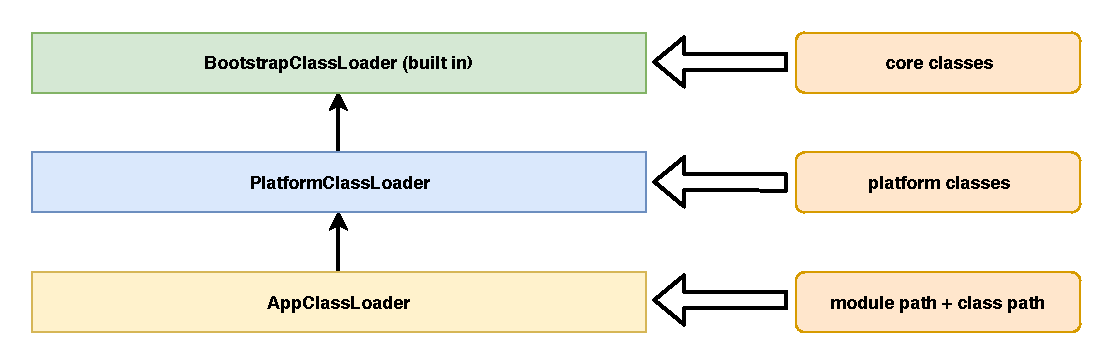
\includegraphics[scale=0.7]{assets/AllGraphicsTalk-classloader.pdf}
	\end{center}
\end{frame}

\begin{frame}
	\frametitle{Startup life cycle of a class (Java 11 lang spec)}
	\begin{enumerate}
		\item{Loading §12.2.1}
			\begin{itemize}
				\item{Loading the byte code into the JVM using a class loader}
			\end{itemize}
		\item{Verify §12.3.1}
			\begin{itemize}
				\item{Validation of the class structure / op codes / method signatures, ...}
			\end{itemize}
		\item{Prepare §12.3.2}
			\begin{itemize}
				\item{Storage allocation, initialization of static field (default values, not static initializer!)}
			\end{itemize}
		\item{(Resolve §12.3.3)}
			\begin{itemize}
				\item{Symbolic link resolution (optional step, may be executed lazily)}
			\end{itemize}
		\item{Initialization §12.4.1}
			\begin{itemize}
				\item{Call static initializers, initialization of static fields}
			\end{itemize}
	\end{enumerate}
\end{frame}

\begin{frame}
\frametitle{A word about modules...}
\begin{itemize}
    \item{Since Java 9 each class is member of a module}
    \item{If the class is not being loaded from a module, its placed in an ''automatic module''}
    \item{Classes in auto modules are allowed to do anything like they did before Java 9}
    \item{Rules of the module system only apply to classes loaded from non auto modules}
    \item{Demos in this talk are using classes with auto modules}
\end{itemize}
\end{frame}
\section{Live Coding examples}


%% 1 und 2
\begin{frame}
    \begin{center}
    Lets write some basic code...
    \end{center}
\end{frame}

\begin{frame}
	\frametitle{Webapp classloader delegation model}
	\begin{center}
	    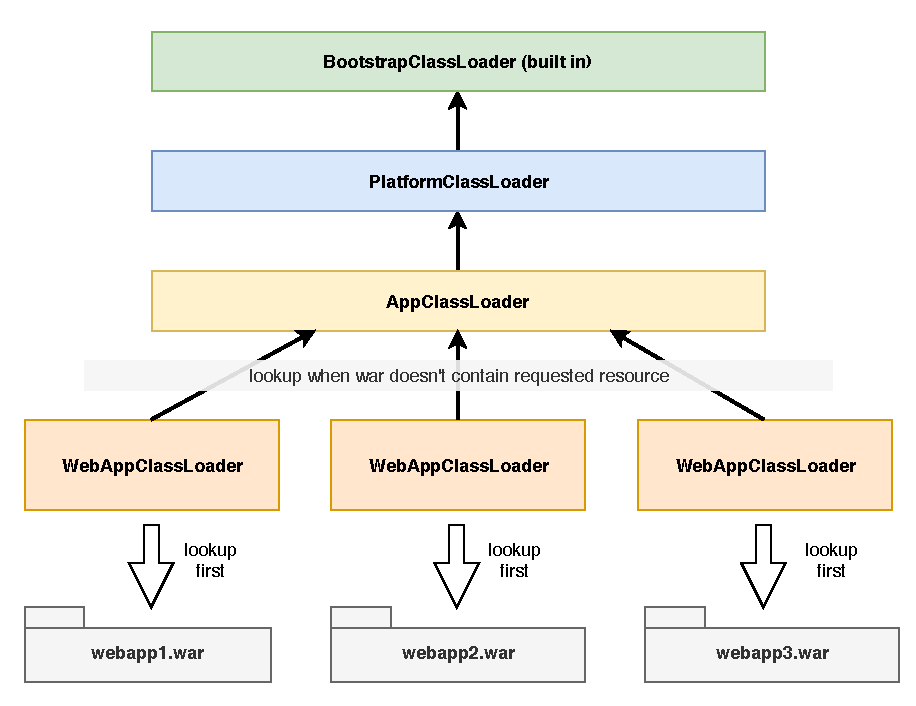
\includegraphics[scale=0.5]{assets/AllGraphicsTalk-webappclassloader.pdf}
	\end{center}
\end{frame}

% Hibernate Example
\begin{frame}
    \begin{center}
    Lets code our own plugin system
    \end{center}
\end{frame}

\begin{frame}
	\frametitle{Hibernate plugin example}
	\begin{center}
	    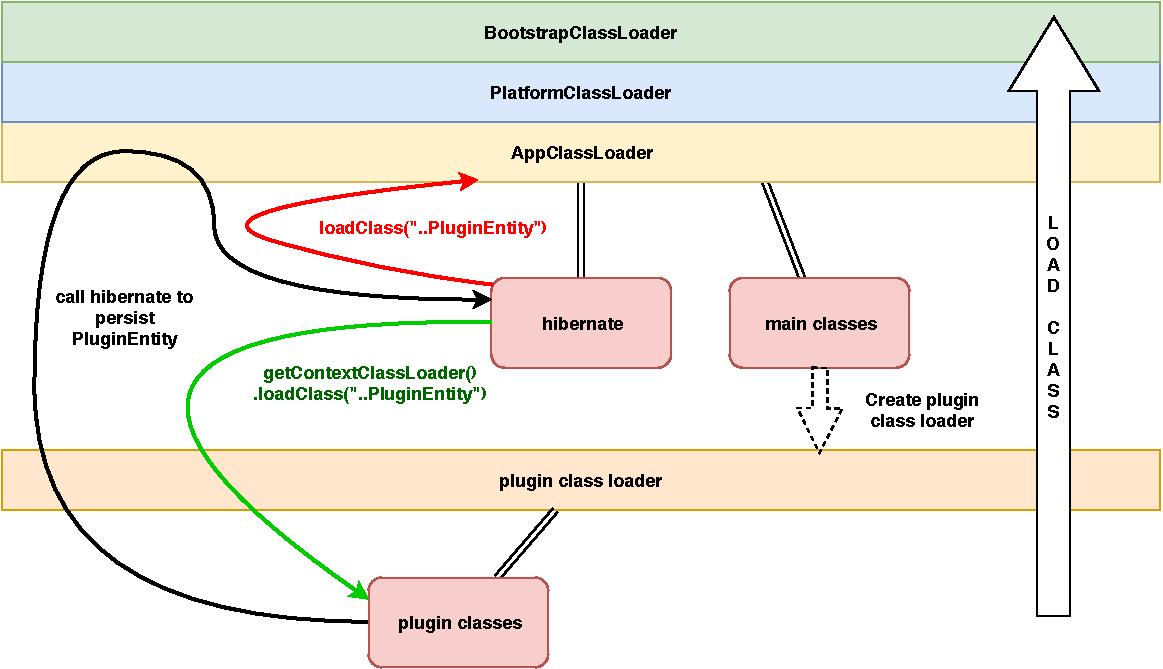
\includegraphics[scale=0.5]{assets/AllGraphicsTalk-hibernate.pdf}
	\end{center}
\end{frame}

\begin{frame}
    \begin{center}
    Lets code a better approach than shading + relocation
    \end{center}
\end{frame}

\begin{frame}
	\frametitle{Fancylib shading example}
	\begin{center}
	    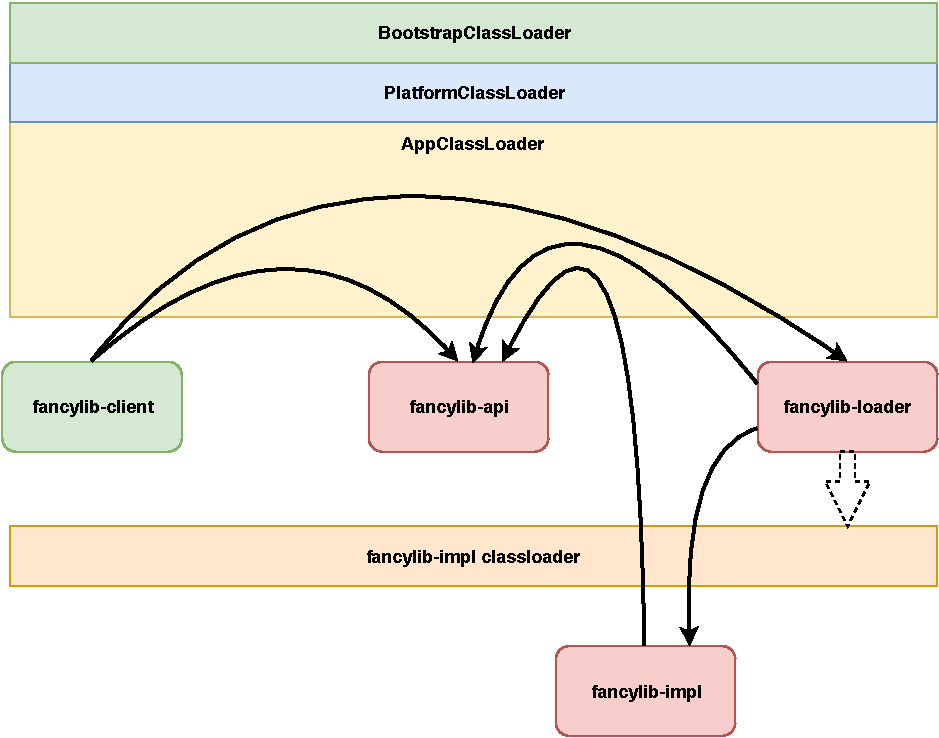
\includegraphics[scale=0.45]{assets/AllGraphicsTalk-shading.pdf}
	\end{center}
\end{frame}

\begin{frame}

\begin{columns}
    \begin{column}{0.25\textwidth}
	\begin{center}	
	\bigskip
	
\includegraphics[scale=0.07]{assets/qrcode-github.pdf}
	\end{center}
    \end{column}

   \begin{column}{0.48\textwidth}
\begin{center}	
        \large{Thank you for your attention!}
\end{center}
    \end{column}

    \begin{column}{0.25\textwidth}
	\begin{center}	
		\bigskip
		
\includegraphics[scale=0.1]{assets/qr-code.pdf}
	\end{center}
    \end{column}
\end{columns}

\end{frame}

\end{document}
